% \documentclass[lineno,twocolumn,endfloat,biblatex]{biophys-new}
\documentclass{biophys-new}
\usepackage[utf8]{inputenc}
\usepackage{graphicx}
\usepackage[colorlinks,allcolors=cyan!70!black]{hyperref}

% uncomment if using biblatex
% \addbibresource{sample.bib}

\usepackage{lipsum}
\usepackage[normalem]{ulem}

\title{Understanding the Free Energy Landscape of Phase Separation in Lipid Bilayers using Molecular Dynamics}
\runningtitle{FLOPSS} %% For page header

\author[1]{Ashlin J. Poruthoor}
\author[1,*]{Alan Grossfield}
\runningauthor{Poruthoor and Grossfield} %% For page header

\affil[1]{University of Rochester Medical Center, Rochester, NY 14620}

\corrauthor[*]{alan\_grossfield@urmc.rochester.edu}

% \papertype{Letters}
\papertype{Article}
% \papertype{Computational Tools}


\begin{document}

\begin{frontmatter}
\begin{abstract}

Liquid-liquid phase separation (LLPS) inside the cell often results in biological condensates that can critically impact
cell homeostasis. Such phase separation events occur in multiple parts of cells, including
the cell membranes, where the so-called ``lipid raft'' hypothesis posits the formation of ordered domains floating in a sea
of disordered lipids. The resulting lipid domains often have functional roles.
However, the thermodynamics of lipid phase separation and their resulting
mechanistic effects on cell function and dysfunction are poorly understood. Understanding such complex phenomenon in cell
membranes, with their diverse lipid compositions, is exceptionally difficult. For this reasons, simple model systems that can recapitulate similar behavior are
widely used to study this phenomenon. Despite these simplifications, the timescale and and length scales of domain formation
pose a challenge for molecular dynamics (MD) simulations.
Thus, most MD studies focus on spontaneous lipid phase separation --- essentially measuring the sign (but not the amplitude) of the free energy change upon separation --- rather than directly interrogating the thermodynamics.  Here, we propose a proof-of-concept pipeline that can 
directly measure this free energy by combining coarse-grained MD with enhanced sampling protocols using a novel collective variable. This approach will be a useful tool to help connect the thermodynamics of phase separation with the mechanistic insights already available from molecular dynamics simulations.


\end{abstract}

\end{frontmatter}

\section*{Introduction}

Interactions among biomolecules often result in phase separation and subsequent formation of biological condensates\cite{Banani2016}.
In the past decade, there has been a new appreciation for the role of phase separation in cell physiology\cite{Banani2017}. Biological condensates involving fundamental biomolecules like DNA\cite{Larson2017}, RNA\cite{Langdon2018}, protein\cite{Li2012}, and lipids\cite{Sezgin2017} have been identified and their functional roles at least somewhat understood.
Biological condensates are involved in diverse processes, including DNA damage response\cite{Altmeyer2015}, translational\cite{Decker2012} and transcriptional\cite{Lallemand-Breitenbach2010} regulation, ribosome biogenesis\cite{Feric2016}, cell adhesion\cite{Case2015}, and endocytosis\cite{Degreif2019}.
Such nano-to-micron-scale compartments have no surrounding membrane but sequester key molecules and help in cellular organization, similar to canonical organelles\cite{Mao2011,Boisvert2007}.
These transient and dynamic sequestration zones are crucial for cell stress responses\cite{Boisvert2007} and signal transductions\cite{Janosi2012}.
As phase-separated molecules are concentrated within these condensates, they can function as reaction crucibles that enhance reaction kinetics\cite{Strulson2012}.
However, abnormal phase behavior of biological condensates is speculated to underlie multiple disease states, including neurodegenerative diseases such as Huntington's\cite{Li2016}, ALS\cite{Jain2017}, and Parkinson's\cite{Ray2020}.


Like these intracellular biological condensates, phase separation in the cell membrane often results in relatively ordered lipid lateral domains with collective behavior that can recruit other proteins and lipids\cite{Sezgin2017, Case2019}.
Such domains often cluster signaling molecules\cite{Tian2007} and facilitate conformational modulations through domain-specific lipid interactions\cite{Laganowsky2014,Lingwood2011} that are relevant in immune signaling\cite{Beck-garcia2015,Wisser2017} and host-pathogen interactions\cite{Dick2012}.
As membrane properties modulate resident protein function, the coexistence of distinct phases gives the cell an extra tool for regulation.
Conformational changes in domain-resident molecules and their subsequent activity shifts regulate key signaling events\cite{Laganowsky2014,Lingwood2011}.
It has also been observed that the HIV Gag protein is sensitive to domains with high cholesterol content, suggesting a potential role of membrane domains in host-pathogen interaction and viral assembly\cite{Dick2012}.
Moreover, lipid domains are conserved throughout the tree of life, implying their relevance in regulating cellular processes\cite{Sezgin2017}. 
For these reasons, understanding the thermodynamics of lipid phase separation as a function of the composition of the system is a critical step toward understanding the molecular grammar behind lipid domains and the resultant functional modulations. 


Lipid domains have been studied extensively both experimentally and computationally.
However, teasing out the complex interactions between domain components that determine the membrane organization is challenging in vivo due to the limitations of different methodologies\cite{Klotzsch2013}.
Such difficulties primarily arise due to (a) the complex composition of cell membrane\cite{Tieleman2019}, (b) difficulties in defining domain properties in vivo\cite{Sezgin2017}, and (c) challenges in achieving specificity when perturbing the system with probes\cite{Veatch2007}.
Hence, simple model membranes have been extensively used to mimic the phase separation of complex cell membrane phenomenon in vitro\cite{Veatch2003a,Veatch2002,Veatch2003} and in silico\cite{Risselada2008,Lin2016,Lin2019}.
Such studies provide powerful insights into phase-separated domains, their properties, and whether the process is favorable, but as a rule they cannot quantify the underlying thermodynamics. This limits our ability to assess the contributions of different mechanistic effects to the process.

As a ``computational microscope\cite{Dror2012}'', molecular dynamics (MD) simulations have been used to study spontaneous lipid separation without using exogenous labels or probes\cite{Pantelopulos2018}.
However, MD simulations designed for spontaneous phase separation are inadequate to compute thermodynamic properties with statistical confidence.
This is because the transition between mixed and separated states is often a single irreversible event on the microsecond timescale typically achievable by typical all-atom or even coarse-grained MD\cite{Risselada2008,Bennett2018}, especially given the
the relatively large size required to model the phenomenon. 
That said, CG-MD is an excellent tool to study phase separation in the membrane, because it retains molecular-level resolution while capturing nanoscale domains due to transient phase separation events.

Previously, the Tieleman\cite{Bennett2018} and the Gorfe groups\cite{Lin2019} have done some pioneering work on the thermodynamics of lipid domains.
While the former used thermodynamic integration\cite{Salsburg1953} to calculate the free energy and excess chemical potential for exchanging lipid species between phases, the latter used umbrella sampling\cite{TorrieG.MValleau1977} to compute the membrane partition thermodynamics of an idealized transmembrane domain by dragging it across the boundary between distinct lipid phases.

We hypothesize that coupling a more versatile enhanced sampling method with the standard CG-MD will improve the transition events between the mixed and separated states of the lipid bilayer system under study to compute the free energy for phase separation.
Various enhanced sampling protocols have previously demonstrated their ability to enhance the sampling of rare events\cite{Henin2022}.
In most cases, external forces are applied to the system to bias simulation to explore the desired phase space.
As a result, it is necessary to compute the derivative of the collective variable at each time step.
Certain popular implementations of such protocols, like COLVARS\cite{Fiorin2013} and PLUMED\cite{Barducci2015}, are done on single CPUs serially, leading to poor performance when the collective variable is computationally complex, as is the case for the complicated collective variables proposed to study phase separation.

By contrast, the weighted ensemble (WE)\cite{Huber1996, Zuckerman2017} method has the advantages of (a) unbiased dynamics, and (b) good sampling, achieved by enhancing the sampling of otherwise undersampled phase space and reducing the sampling of otherwise oversampled phase space.
Moreover, there is an added benefit, in that the calculation of the collective variable can be decoupled from the MD, which simplifies its implementation and can improve the computational performance.
It should be noted that the WE method is highly parallelizable and can take advantage of GPU acceleration\cite{Zwier2015}.

Here we present a novel proof-of-concept pipeline to estimate the equilibrium free energy change upon separating a lipid bilayer into distinct coexisting phases.
We test this pipeline on three different lipid bilayer systems with varying degrees of phase separation propensity.
We explore three potential candidate collective variables and assess their effectiveness in the pipeline.
We then construct free energy landscapes of the three systems at multiple temperatures.
We further explore a few non-traditional use cases for the data thus generated and discuss additional room for improvements.

\begin{figure}[hbt!]
\centering
\includegraphics[width=6.25in]{Figures/Main/1/Final/placeholder.jpg}
\caption{A. 2D structure and corresponding MARTINI 2 bead structure for lipids used in this study. B. Time evolution of each lipid system as a function of time. The membrane normal is pointing towards the reader.}
\label{fig1:view}
\end{figure}

\section*{Methods}

\subsection*{System details}

As shown in Fig \ref{fig1:view}, we used three different ternary lipid bilayer systems:
1. A lipid bilayer consisting of dipalmitoyl-phosphatidylcholine (DPPC), dilinoleyl-phosphatidylcholine (DIPC), and cholesterol (CHOL), known to phase separate in silico in a few microseconds \cite{Risselada2008, Schafer2010, Janosi2012, Doma2012, Jong2013, Liu2020, Su2020}.
2. A lipid bilayer consisting of DPPC, diarachidonoyl-phosphatidylcholine (DAPC), and CHOL, known to phase separate in silico within a few hundred nanoseconds \cite{Lin2016, Lin2019, Davis2013a}.
3. A lipid bilayer consisting of DPPC, palmitoyl-oleoyl-phosphatidylcholine (POPC), and CHOL that was previously shown not to phase separate \cite{Veatch2003,Davis2013a}.
The composition of the DPPC-DIPC-CHOL, DPPC-DAPC-CHOL, and DPPC-POPC-CHOL systems used here are (0.42/0.28/0.3), (0.5/0.3/0.2) and (0.4/0.4/0.2) respectively and are adapted from previous studies \cite{Risselada2008, Lin2016, Davis2013a}.
We kept the total number of lipids the same as in previous calculations as well, with the  DPPC-DIPC-CHOL, DPPC-DAPC-CHOL, and DPPC-POPC-CHOL systems containing 1944, 1200 and 1200 respectively. 

Due to the relatively large system sizes and the time scale required for phase separation and related dynamics in lipid bilayer simulations, we used a coarse-grained (CG) model for each system. Although nothing in the subsequent sampling or analysis is specific to the coarse-grained models, it makes sense to use a less expensive model while working out the method.
 
Using CHARMM-GUI Martini Maker \cite{Qi2015}, we constructed four replicas of each CG ternary symmetric bilayer system, with the lipids randomly mixed in the bilayer.
We used MARTINI 2 force field parameters and particle definitions\cite{Marrink2007, DeJong2013} to construct CG systems and to run the subsequent MD simulation.
We replaced the default input files from CHARMM-GUI Martini Maker with their respective most recent Martini 2.x versions if they existed.
We used the MARTINI polarizable water model\cite{Yesylevskyy2010} to solvate all systems with approximately a 1:30 lipid to real water ratio.
A detailed description of the systems is given in Table S1 of supplementary material.
We did not use the more recent MARTINI 3.0 lipid parameters, since there are no published MARTINI 3 parameters for cholesterol at this time.

\subsection*{Standard MD simulation details}

We used GROMACS 2020.3\cite{Abraham2015} to propagate the dynamics of the systems prepared. 
Each system was minimized and equilibrated following the protocol suggested by CHARMM-GUI Martini Maker.
To obtain an intact bilayer without any membrane undulations, we used  
the flat bottomed restraint potential available in GROMACS; this allowed the lipids to move freely in the plane of the membrane but restrained within a slab of defined $z$ thickness along the membrane normal.  
More details about membrane restraining protocol are given in the supplementary material (section 2).

After the minimization and equilibration, all systems were run at 400 K in the NPT ensemble for 100 ns to make sure the lipids in each system were randomly distributed.
For every system, we forked each replica into multiple temperature runs simulated at different temperatures ranging from 298K to 450K.
For these production runs, the temperature coupling is done using velocity rescaling\cite{Bussi2007} with a time constant 1 ps.
An extended-ensemble Parrinello-Rahman pressure coupling\cite{Parrinello1981} with a relatively high time constant of 12 ps was used, as recommended for MARTINI.  A semiisotropic pressure coupling suited for membrane simulations is used here with a compressibility of 3$\times 10^{-4}$ $\text{bar}^{-1}$ and reference pressure for coupling as 1 bar.
A reaction field electrostatics with Coloumb cutoff of 1.1 nm was used, and 
a dielectric constant of 2.5 was used, as required with the MARTINI polarizable water model.
For Van der Waals interaction, a similar cutoff of 1.1 nm was used.
A potential-shift Van der Waal modifier was also used.
For neighbor searching, a verlet cutoff scheme was used with neighbor list updated every 20 steps.
The simulation parameters were mostly inspired by previous CG MARTINI simulations\cite{DeJong2016}. 
To eliminate potential artifacts previously reported due to inaccurate constraints\cite{Javanainen2020}, we used an 8th order expansion for the LINCSolver constraint coupling matrix\cite{Hess1997} for more accuracy.
Moreover, for better energy conservation, we also used short 20 fs timesteps, which is conservative for a CG system.

All standard MD simulations ran for at least 8 microseconds using the BlueHive supercomputing cluster of the Center for Integrated Research and Computing at the University of Rochester.
Simulations ran on Intel Xeon E5-2695 and Gold 6130 processors augmented with Tesla K20Xm, K80, and V100 GPUs.   
The trajectories were processed and analyzed using the LOOS software package\cite{Romo2014}.
A detailed description of the simulation parameters is given in Table S1 of supplementary material. 

\subsection*{Collective Variables}

A collective variable is a reduced coordinate that captures the progress of a system along the transition of interest.
Ideally, such a reduced variable(s) should fully capture the key modes of the system to reflect the complex event under study.
The success and efficiency of any enhanced sampling protocol depends on the chosen collective variable over which the sampling is enhanced\cite{Valsson2016, Yang2019b, Henin2022}. 
We explored 3 candidate collective variables for the WE simulations.

\subsubsection*{1. Fraction of Lipids in Clusters (FLC)}
Since the formation of lipid domains with distinct properties from the rest of the bilayer is a characteristic feature of a phase-separating lipid bilayer,
we hypothesized that we could use a variable that quantifies the recruitment of lipids into such domains to track the phase separation events in our systems.
Here, we define the Fraction of Lipids in Clusters (FLC) as follows:

\begin{equation}
\label{eq:FLC}
\text{FLC} = \sum_{i}^{N} \frac{\text{No. of $X_i$ lipids in lipid $X_i$ Clusters}}{\text{No. of Lipid $X_i$}} =  \frac{\sum_{i}^{N} \text{No. of Lipid X$_i$ in Lipid X$_i$ Clusters}}{\text{Total No. of Lipids}}
\end{equation}

\noindent Where subscript $i$ denotes the individual lipid species in a bilayer consisting of N total lipid species.
As shown in Figure \ref{fig2:view}, each system under study has $N=3$ lipid species.
FLC increases as the system goes from a mixed state, with a random distribution of lipids, to a separated state.
An FLC of 0 corresponds to a system configuration where no lipids are part of any cluster,
while an FLC of 1 implies that all lipids are in a cluster (though not necessarily a single cluster).


\begin{figure}[hbt!]
\centering
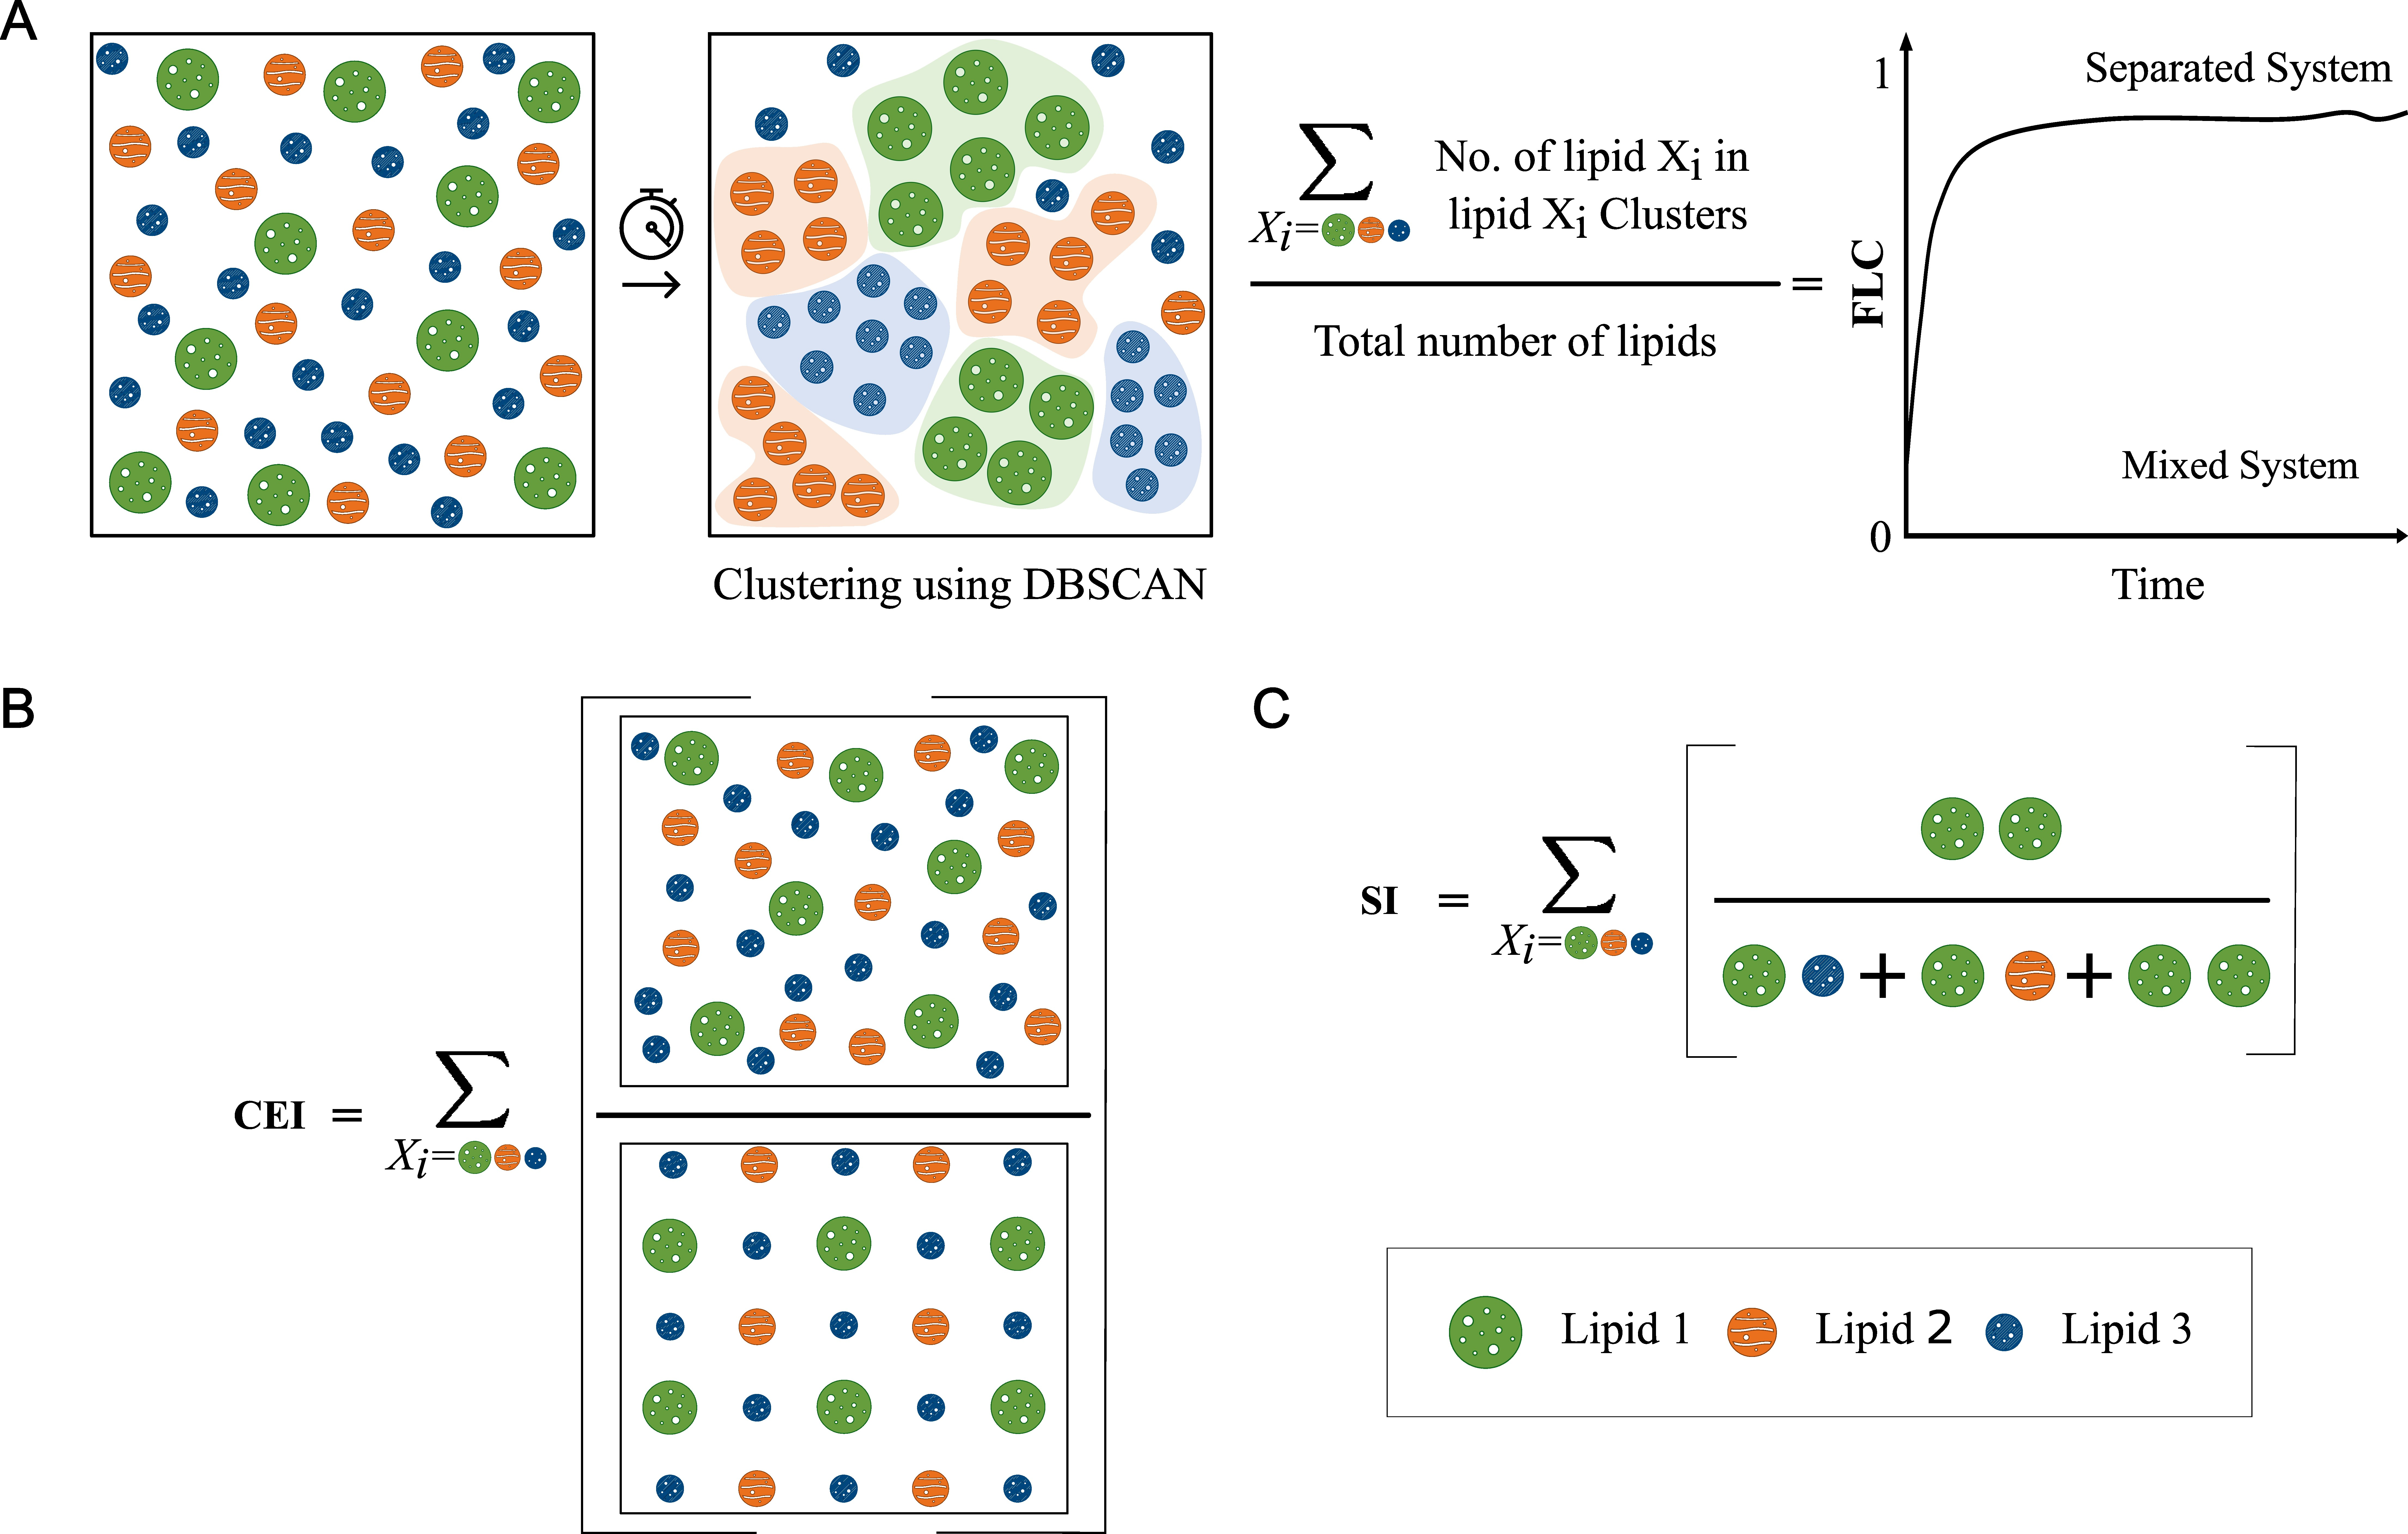
\includegraphics[width=6.5in]{Figures/Main/2/placeholder.jpg}
\caption{A. Illustration of FLC :  Functional form of FLC and expected evolution curve for a phase separating system. B. Illustration of Cumulative Enrichment Index. C. Illustration of Segregation Index}
\label{fig2:view}
\end{figure}


The lipid $X_i$ cluster is defined using the Density-Based Spatial Clustering of Applications with Noise (DBSCAN) algorithm \cite{MartinEsterHans-PeterKriegelJiirgSander1996, Ester2017} as implemented in scikit-learn \cite{PedregosaF.VaroquauxG.GramfortA.MichelV.ThirionB.GriselO.BlondelM.PrettenhoferP.WeissR.andDubourgV.VanderplasJ.PassosA.CournapeauD.BrucherM.PerrotM.Duchesnay2011}.
For lipid DBSCAN clustering, instead of the default euclidean metric to calculate the distance between lipid centroids, we precomputed the 2-dimensional distance matrix adjusted for periodic boundary conditions; the distance calculation was performed using LOOS, with the two leaflets treated independently.
The DBSCAN algorithm requires two additional input parameters: $min\_samples$ and $\varepsilon$.
We consider lipids with more than $min\_samples$ neighbors (including the lipid itself) within $\varepsilon$ radius as core lipids.
Non-core lipids still within $\varepsilon$ radius of a core lipid are considered border lipids.
A set of core lipids within $\varepsilon$ radius of each other and their border lipids forms a cluster.
All lipids that are not a part of any cluster are considered outliers.

Since lipid motion in a bilayer is constrained primarily on a plane and MARTINI beads for a lipid are of similar radii, we can use the two-dimensional version of Kepler's conjecture that the densest packing of unit disks in a plane is hexagonal close packing (Thue's Theorem).
Hence we chose 7 (6 nearest neighbors + 1 central lipid) as $min\_samples$ for all the lipid species.
However, $\varepsilon$ was chosen differently for each lipid species based on their first nearest neighbor distance from the central lipid.
We used the $xy\_rdf$ tool in LOOS to calculate an individual lipid species' first nearest neighbor distance.
From the first 8 $\mu$s MD standard simulation of each replica, we computed the radial distribution function (RDF) for a lipid species in the xy-plane. 
From the RDF plot, we found the first maxima (provided it is above 1), and the distance to the minima right after this first maximum was determined to be the first nearest neighbor distance for that lipid species.
This distance was averaged over all four replicas for a given system at a given temperature and then assigned as the respective $\varepsilon$ input.
Since nearest neighbor distance is a function of temperature, for the same lipid species in the same system, $\varepsilon$ may be different for different temperatures.
The computed $\varepsilon$, i.e., average first nearest neighbor distance for different conditions, are plotted in Supplementary Figure S1.
Additionally, we tracked auxiliary variables (AVs) that evaluate the quality of DBSCAN clustering since it is critical for defining the FLC that drives the WE equilibrium dynamics (Supplementary section 4, Figures S2-S5).

\subsubsection*{2. Cumulative Enrichment Index (CEI)}

When lipids segregate into phases, one result is that the local concentration of a given lipid type in the vicinity of other lipids of the same type is increased. We attempted to exploit this phenomenon by tracking the degree of local lipid enrichment, similar to other methods previously used \cite{Gu2019, Gu2020}.
Here, we calculated the average local density of $X_i$ lipids around a single lipid $X_{ij}$, within a cutoff radius, $\epsilon_i$, defined as above for FLC estimation.
We defined a normalization factor, $\Phi_i$, as the local density of $X_i$ lipids for a uniformly well-mixed system of similar composition.
The ratio of former respective to latter forms the enrichment index for a lipid species, $X_i$.
CEI is defined as the sum of individual enrichment index for all the lipid species in the system, as follows:

\begin{equation}
    \begin{aligned}
    \label{eq:CEI}
    \text{CEI} {}   & = \sum_{i}^{N}\Bigg[\frac{\text{Average local density of lipids $X_i$ around a single lipid $X_i$}}{\text{Local density of lipid $X_i$ for a well mixed system}}\Bigg]_{\text{$\epsilon_i(T)$}} \\
                    & =  \sum_{i}^{N} \frac{1}{\Phi_i}\frac{1}{\text{$\pi\epsilon_i^2$}}\sum_{j}\text{No. of $X_i$ lipids around $X_{ij}$ lipid in $\epsilon_i(T)$ radius}
    \end{aligned}
\end{equation}

Where $X_{ij}$ denotes $j^{th}$ lipid of $X_i$ lipid species.
The local density around $X_{ij}$ is calculated within $\epsilon_i(T)$ distance, where T is the temperature of the system, corrected
for the contribution of the central lipid.
For the normalization factor, $\Phi_i$,  we calculated the global density of $X_i$ lipids by taking the ratio of the total number of $X_i$ lipids in the system to the $xy$-planar area of the bilayer system.
This global density is the same as the local density of $X_{i}$ lipid for a uniformly well-mixed system.
Thus CEI significantly larger than 3 implies that the ternary system, $N=3$, deviates from a well-mixed state to a separated state.

\subsubsection*{3. Segregation Index (SI)}

We defined a contact-based quantity to track the homogeneity of the lipid bilayer, similar to the ones that track the mixing of beads used previously\cite{Marigo2012, Kumar2020}.
Here, we computed the total contacts between a given lipid and its environment and computed the fraction of the those contacts to like-species lipids:

\begin{equation}
    \begin{aligned}
    \label{eq:CLT}
    \text{SI} = \sum_{i}^{N}\Bigg[\frac{X_iX_i}{\sum_{j}^{N}X_iX_j}\Bigg]_{\text{$\epsilon_i(T)$}} = \frac{X_{11}}{X_{11} + X_{12} + X_{13}} + \frac{X_{22}}{X_{21} + X_{22} + X_{23}} + \frac{X_{33}}{X_{31} + X_{32} + X_{33}}
    \end{aligned}
\end{equation}

$X_iX_j$ denotes the contacts between lipid species $X_i$ and $X_j$ within $\epsilon_i(T)$ cutoff.
Thus for a ternary bilayer system, SI $=$ 3 implies a fully separated system, and SI $<$ 3 implies mixing.
However, for the analysis, we ignored the contribution of cholesterol as we found that excluding the cholesterol term did not change the functional behavior (Supplementary Figure S6).
Hence, $\text{SI}_{\text{noCHOL}}$ effectively will have bounds [0, 2] unless otherwise stated.    

\subsection*{Weighted Ensemble Simulation}

\subsubsection*{Preparing seeding configurations for WE simulation} 
From each 8 $\mu$s MD simulation of a given composition, the last ten frames spaced by 100 ns were collected.
These structures contained mixed and unmixed states, which we used as starting structures to begin the weighted ensemble simulations; starting the WE with structures scattered across the collective variable range reduces the time needed to generate well-equilibrated free energy curves.

For the DPPC-DAPC-CHOL and DPPC-DIPC-CHOL systems, the set of mixed configurations for a particular replica came from the respective 423 K and 450 K simulation frames, since both systems are only well-mixed at high temperatures.
The set of separated configurations for a replica comes respectively from the 298K and 323K simulations.
For the DPPC-POPC-CHOL system, starting structures were taken from the 298K and 450K trajectories; although the system never phase separates, using these two temperatures gives structures that span the whole range of the collective variables.

\subsubsection*{Running WE simulations} 
We ran weighted ensemble equilibrium simulations using version 1.0 of the WESTPA package\cite{Zwier2015}, closely following the previously established protocol\cite{Bogetti2019}.
The collective variable was divided into 30 dynamic bins using the minimal adaptive binning scheme (MAB)\cite{Torrillo2021}.
For each replica, a target number of 4 short simulations, or ``walkers'' per bin, were started in parallel from the mixed and the separated configurations prepared earlier.
After every resampling interval of 1 ns, the collective variable was evaluated to initiate the merging and splitting of walkers to maintain the target number of walkers per bin. One cycle of MD and resampling is referred to as a single WE iteration. 
We conducted 500 WE iterations for each replica.
We used GROMACS 2020.3 to propagate the dynamics, using the same parameters described earlier for the standard MD simulations.
The WE Equilibrium Dynamics (WEED) reweighting protocol\cite{Bhatt2010, Suarez2014}, implemented in WESTPA 1.0, was used to accelerate the convergence of WE walkers toward equilibrium.
The reweighting is done every 10 WE iterations.
Four independent WE replicas, started with a different subset of initial structures, were simulated for each temperature and lipid composition. 
All WE simulations were runu sing the Intel Xeon E5-2695 and Tesla K20Xm GPUs in the BlueHive supercomputing cluster of the Center for Integrated Research and Computing at the University of Rochester.   

\subsubsection*{Analysis of WE simulations}
The probability distributions for the CVs for each replica, as a function of WE iterations, were constructed using $w\_pdist$ and $plothist$ tools in WESTPA.
Using this distribution, we monitored the evolution of each WE replica simulation and the convergence.
We used the $w\_multi\_west$ tool in WESTPA to combine data from four the WE replicas of a system at a given temperature.
We then constructed the respective free energy surface from the combined probability distribution of a system. Unless otherwise noted, equilibrium curves were always calculated using the last 10 iterations of each WE run, because combining results pre- and post-reweighting is not statistically correct.
To check the populations in different states and the determine flux between states the $w\_ipa$ tool was used.
When performing this calculation for the DPPC-DIPC-CHOL system at 323K, we defined the states based on visual inspection of the corresponding free energy curves. We defined the mixed and separated states as CEI = [0.0, 3.9] and [4.4, 6.0], $\text{SI}_{\text{noCHOL}}$ = [0.0, 1.3] and [1.4, 2.0], and FLC = [0.0, 0.575] and [0.65, 1.0] respectively.
The choice is arbitrary but reasonable enough to give us a picture of what is happening. 

Input files, initial structures, and scripts required to run and analyze all simulations are available on GitHub at \href{https://github.com/Poruthoor/Phase\_Separation\_Article/tree/main/FLOPSS}{https://github.com/Poruthoor/Phase\_Separation\_Article/tree/main/FLOPSS}

\section*{Results}

Consistent with previous studies from which they are adapted, the standard CG MD simulations of DPPC-(DA/DI)PC-CHOL systems phase separates into $\text{L}_{\text{o}}$ and $\text{L}_{\text{d}}$ regions.
The $\text{L}_{\text{o}}$ region is enriched in the saturated lipid, DPPC, and cholesterol, while the  
$\text{L}_{\text{d}}$ region contained mostly the unsaturated lipids, DAPC or DIPC, depending on the system.
As expected, the DPPC-POPC-CHOL system did not form distinct phases based on visual inspection.
This section compares how different variables track phase separation propensity in lipid bilayers using standard CG MD simulations.
We then compare the convergence of WE simulation to the choice of collective variable.
Finally, we present the free energy landscapes of lipid bilayer systems obtained using WE simulations and discuss reusing the data generated to form other intuitions and applications.

%\subsection*{Tracking phase separating lipid bilayers}

\begin{figure}[hbt!]
\centering
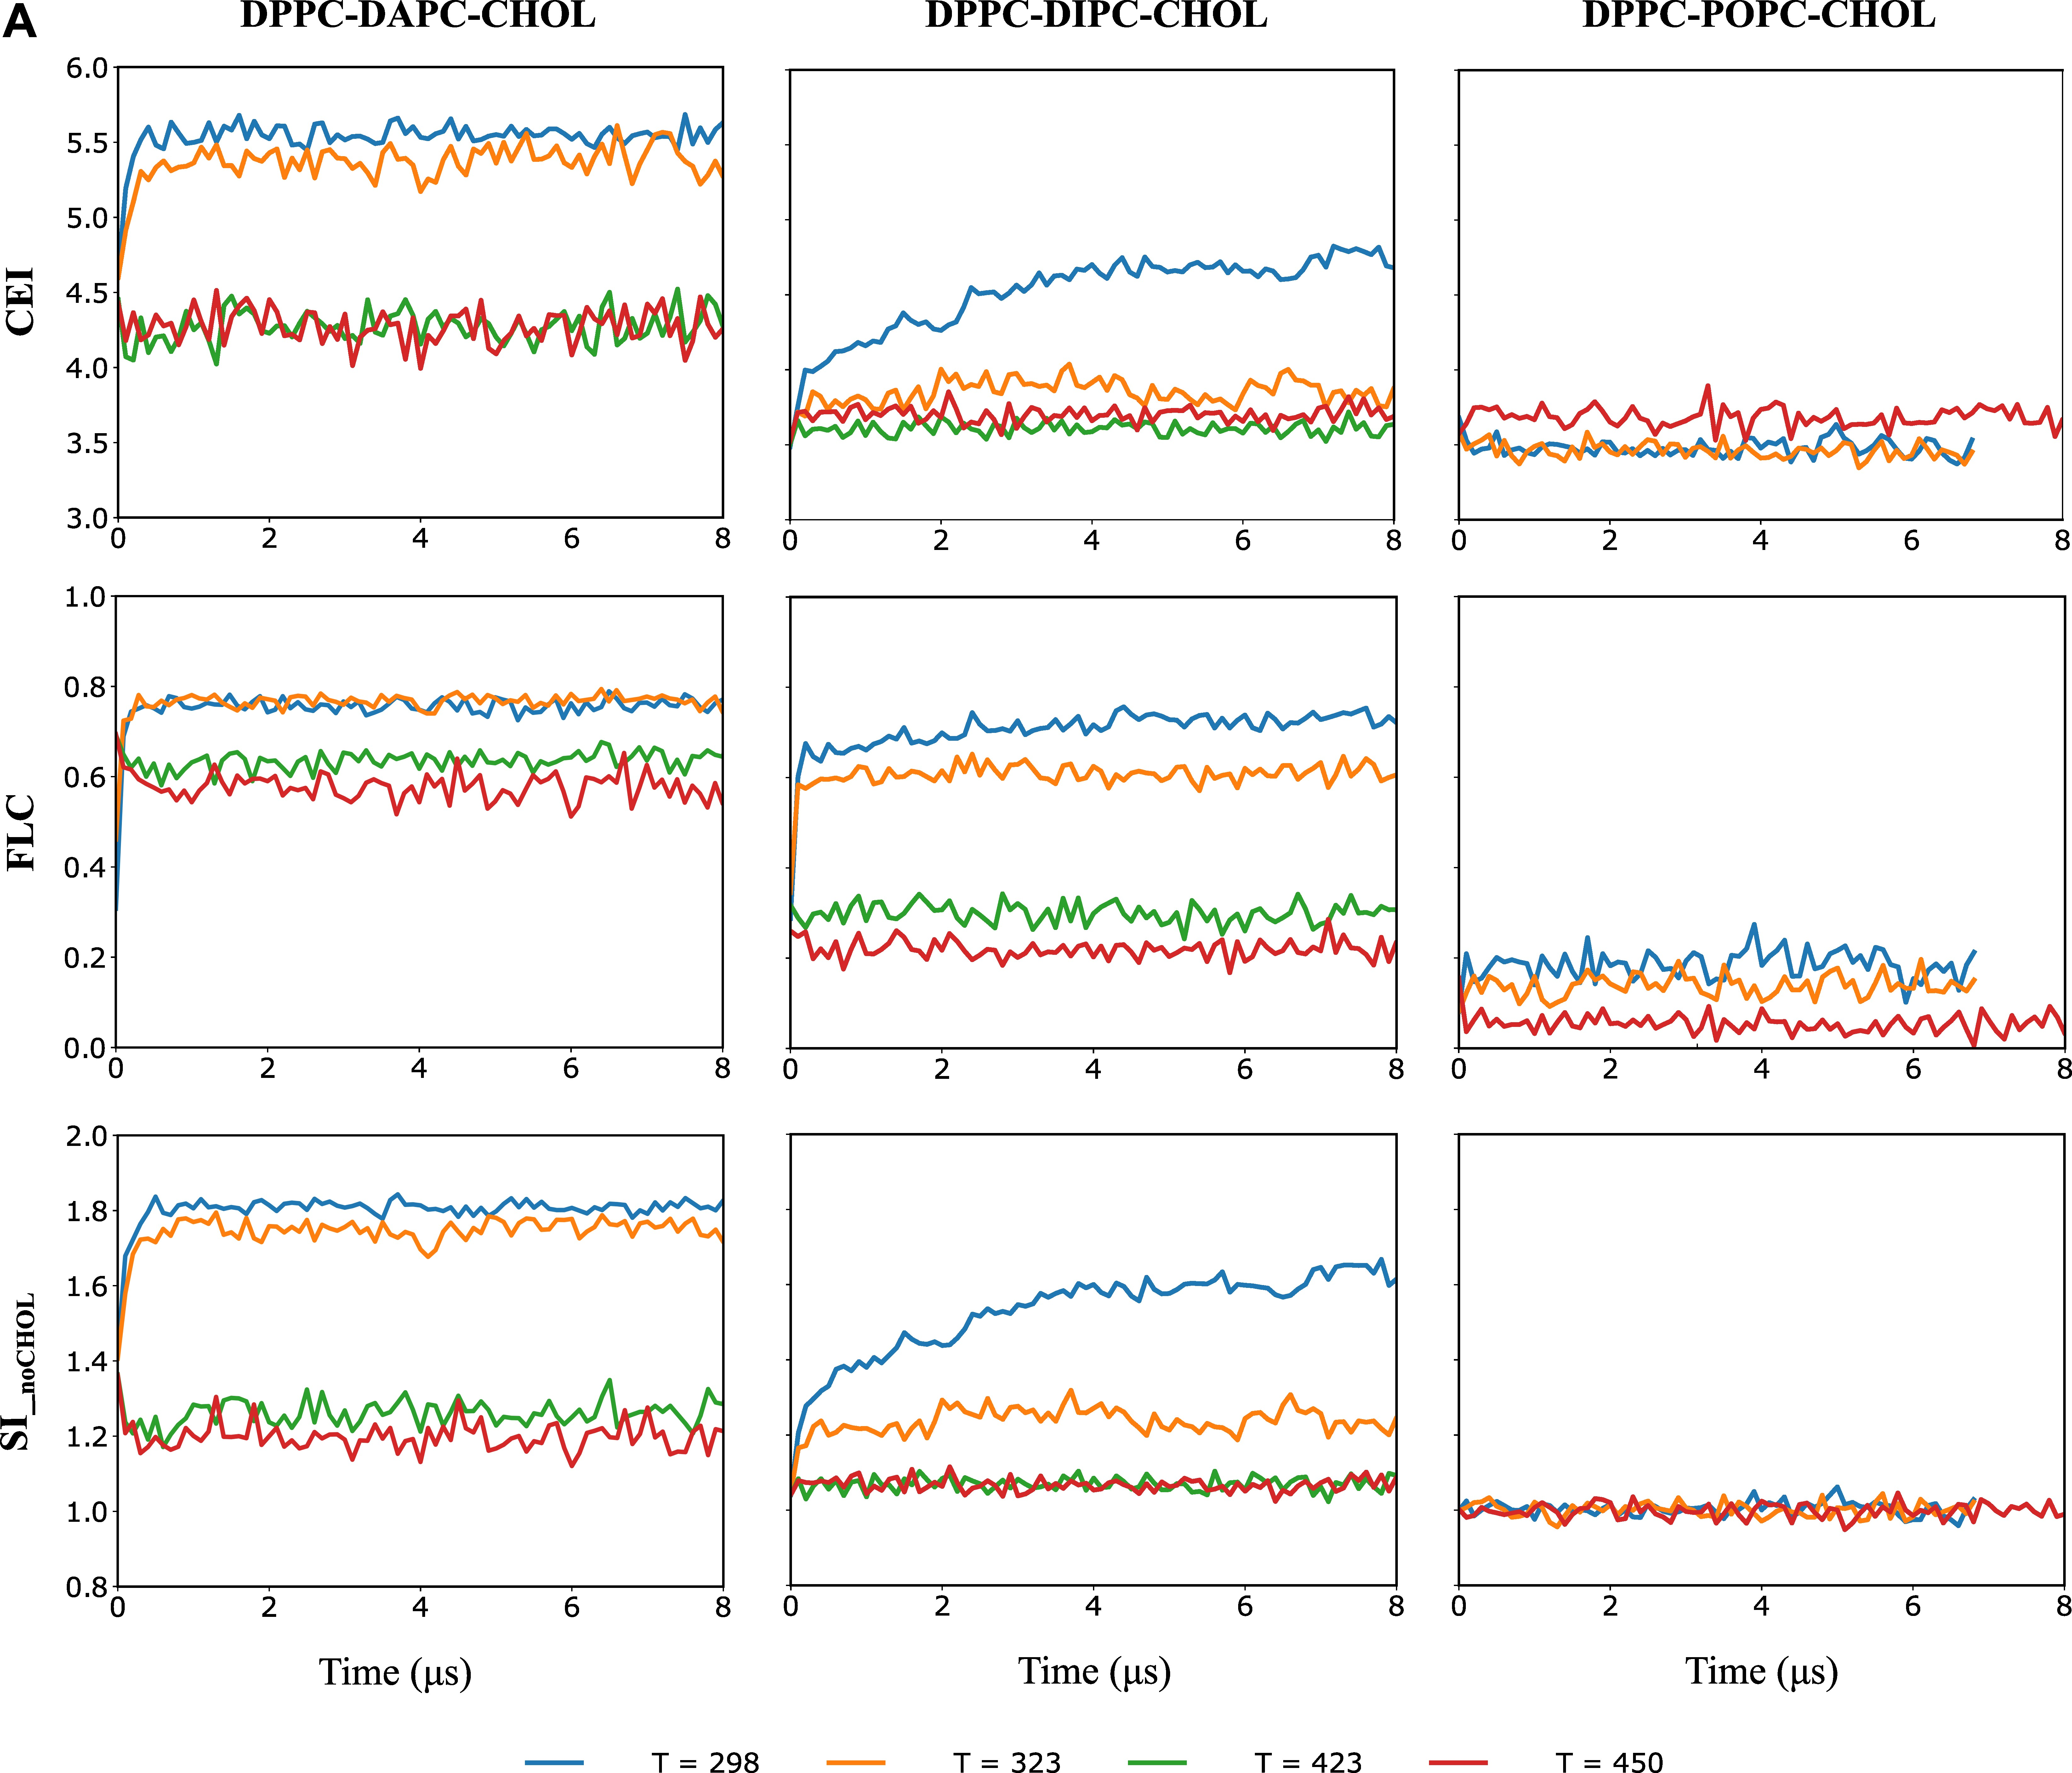
\includegraphics[width=6.5in]{Figures/Main/3/placeholder.jpg}
\caption{A. Time series for three collective variables tracking membrane separation. Each line represents one conventional MD simulation started from a well-mixed state. Each column contains trajectories from a single lipid composition, while each row shows a different variable; 8$\mu$s trajectories were used for all rows. The lines are colored to represent different simulation temperatures.}
\label{fig3:view}
\end{figure}

To evaluate how the collective variables track phase separation, we traced the time evolution of each variable for each system using standard MD starting from well-mixed bilayers.
Figure \ref{fig3:view} illustrates the temporal evolution of FLC, CEI, and $\text{SI}_{\text{noCHOL}}$ for all systems at 298K, 323K, 423K, and 450K.
For the two phase separating systems, the variables capture a single transition between a mixed state and a separated state.
Interestingly, for the relatively slow-separating DPPC-DIPC-CHOL system, CEI and $\text{SI}_{\text{noCHOL}}$ appear to indicate a slower transition than FLC, indicating that while these variables are correlated, they do not measure precisely the same phenomenon.
For the DPPC-POPC-CHOL system, the variables capture a single state corresponding to a mixed system and no transition.
Nevertheless, it is worth noting that FLC, CEI, and $\text{SI}_{\text{noCHOL}}$ capture the effect of temperature in all systems, including for POPC, the negative control, that does not phase separate.

These variables even capture the subtle differences in phase-separating propensity between systems.
For example, at 298K, the plateaued region of the FLC, CEI, and $\text{SI}_{\text{noCHOL}}$ curves are higher for the DPPC-DAPC-CHOL system than the DPPC-DIPC-CHOL system.
This is expected as (a) the lipid chain mismatch between saturated and unsaturated lipid species and (b) the number of double bonds in unsaturated lipid species is high in the DPPC-DAPC-CHOL compared to DPPC-DIPC-CHOL system.
Both these factors have previously been shown to influence lipid phase separation kinetics and domain stability\cite{Fowler2016, Lin2016}.
Thus we have a set of low-dimensional variables that can (a) represent the global dynamics of the lipid bilayer system,
(b) distinguish and track the transition between mixed and separated states, and (c) capture temperature effects,
based on the composition of the system.

\subsection*{Choice of collective variables for WE simulations}

\begin{figure}[hbt!]
\centering
\includegraphics[width=6.5in]{Figures/Main/4/placeholder1.jpg}
\caption{For the given DPPC-DIPC-CHOL replica: A. Free energy curves as a function of WE iteration blocks used to generate them. B. Each plot gives the evolution of configurational distribution for a given collective variable. C. Flux profile between states. The peaks represent crossing of walkers. D. Corresponding state population. Here, each column represent the collective variable that was used to drive WE simulation (FLC, CEI, and $\text{SI}_{\text{noCHOL}}$).}
\label{figs4:view}
\end{figure}

Since CEI, $\text{SI}_{\text{noCHOL}}$, and FLC all track bilayer lipid separation similarly,
we decided to test them as progress coordinates to drive the WE simulation.
Much to our surprise, the 3 coordinates perform very differently.
Figure \ref{figs4:view}A shows free energy curves computed for each coordinate using the DPPC-DIPC-CHOL system at 323K; each curve on a given plot was computed from a different block of 10 WE iterations for the same simulation. The free energy curves generated using CEI and $\text{SI}_{\text{noCHOL}}$ are noisy and not self-consistent, indicating that at best there is poor statistical convergence despite the relatively lengthy 500-iteration WE runs. The $\text{SI}_{\text{noCHOL}}$ runs are still more troubling, in that they suggest that the well-mixed state is favored over the separated one, which contradicts the results from the conventional MD simulations. By contrast, the free energy curves generated using FLC as the collective variable are quite self-consistent, with the phase-separated state slightly favored.
Interestingly, if we monitor the evolution of the free energy curves as a function of WE iterations, shown in Fig \ref{figs4:view}B, the simulations appear to have converged in the sense that they are no longer systematically changing.

These conflicting results raise the following questions: Why do variables that make sense while tracking the system in standard CG MD simulation yield inconsistent or incorrect free energy landscapes when used as collective variables in a  WE simulation?  One clue to diagnose the problem lies in our starting states. In contrast to most WE calculations, which begin the simulation with all walkers in the ``first'' bin, we started with diverse states from across the whole range of the collective variable. While the free energy curves evolve as the WE proceeds, the relative probability of the 2 states remains almost entirely unchanged.

Figure \ref{figs4:view}C confirms this hypothesis by tracking the probability flux between the two states for each coordinate; the results confirm that when CEI or $\text{SI}_{\text{noCHOL}}$ are used as progress coordinates, there is essentially no flux across the barrier separating the separated and mixed states; the flux is literally 0 for CEI, while $\text{SI}_{\text{noCHOL}}$ shows very small fluxes during the last 100 iterations. By contrast, WE simulations using FLC as the coordinate consistently show flux between the two states that is at least several orders of magnitude larger.

Figure \ref{figs4:view}D shows this information another way, tracking the relative population of the mixed and separated states over the course of the WE runs; for clarity purposes the states are defined to exclude the ``middle'' of the coordinate (see the methods section for details), so the state populations do not necessarily add to 1.
It is interesting to note that for CEI, we see a significant drop in the population of the mixed state during iterations 290-300, without a concomitant rise in the other state.
Since our state definition we chose does not span the entire collective variable space leaving a room for the barrier that separates two states, this indicates that some walkers transitioned out of the mixed state, but remained trapped in the middle of the collective variable and never transitioned to separated state. 

For reasons that are not entirely clear, one coordinate (FLC) is far more efficient at sampling transitions than the other two. CEI and $\text{SI}_{\text{noCHOL}}$ do not generate crossing events, and as a result largely recapitulate the probability distribution used to seed the calculation.
The combined results from standard CG MD and WE simulations suggest that CEI and $\text{SI}_{\text{noCHOL}}$ are suitable proxy labels for phase separation but perform poorly as collective variables for sampling.
For this reason, we only continued testing the FLC-based WE calculations for other systems and temperatures.

%\subsection*{Free energy landscapes of lipid bilayer systems}

\begin{figure}[hbt!]
\centering
\includegraphics[width=6.5in]{Figures/Main/5/placeholder.jpg}
\caption{Free energy curves based on FLC-driven WE simulation for three systems. Each line represents a free energy curve, computed as the average of 4 replicate WE runs. Each column contains free energy curves from a single lipid composition. The lines are colored to represent different simulation temperatures.}
\label{figs5:view}
\end{figure}

Figure \ref{figs5:view} shows the free energy profiles of DPPC-DAPC-CHOL, DPPC-DIPC-CHOL, and DPPC-POPC-CHOL lipid bilayer systems.
Each curve is generated by averaging four WE replica simulations, as described in the Methods section, using the last 10 iterations (491-500) of each replica.
Convergence between individual replica free energy curves constructed with last 10 iterations is given in Supplementary Figure S7.
The DPPC-DAPC-CHOL system has a double well behavior at 323K and 353K.
However, both basins correspond to relatively high FLC and appear to be phase separated based on visual inspection.
Even at 423 K, we see that this system prefers to be in configurations where more than 60\% of lipids are in clusters.
For the DPPC-DIPC-CHOL system, the double-well free energy curves gradually shift to the left (fewer lipids in clusters) and change to narrower single-well curves as the temperature increases.
For the DPPC-POPC-CHOL system, the free energy curves at 298K and 423K have a single basin and correspond to a low fraction of lipids preferring to be in any clusters.
In general, FLC-based free energy landscapes capture the role of lipid species constituting the bilayer system in its phase separation.
Moreover, the effect of temperature in decreasing the propensity of a lipid bilayer to separate is evident in all systems.
Although the expectation of clustering-based FLC is to track the formation of domains in a lipid bilayer, the fact that it also neatly captures the temperature effects, even for the negative control POPC system, suggests the robustness of FLC as the collective variable.

\subsection*{Reconstructing free energy landscapes on alternative coordinates}

\begin{figure}[hbt!]
\centering
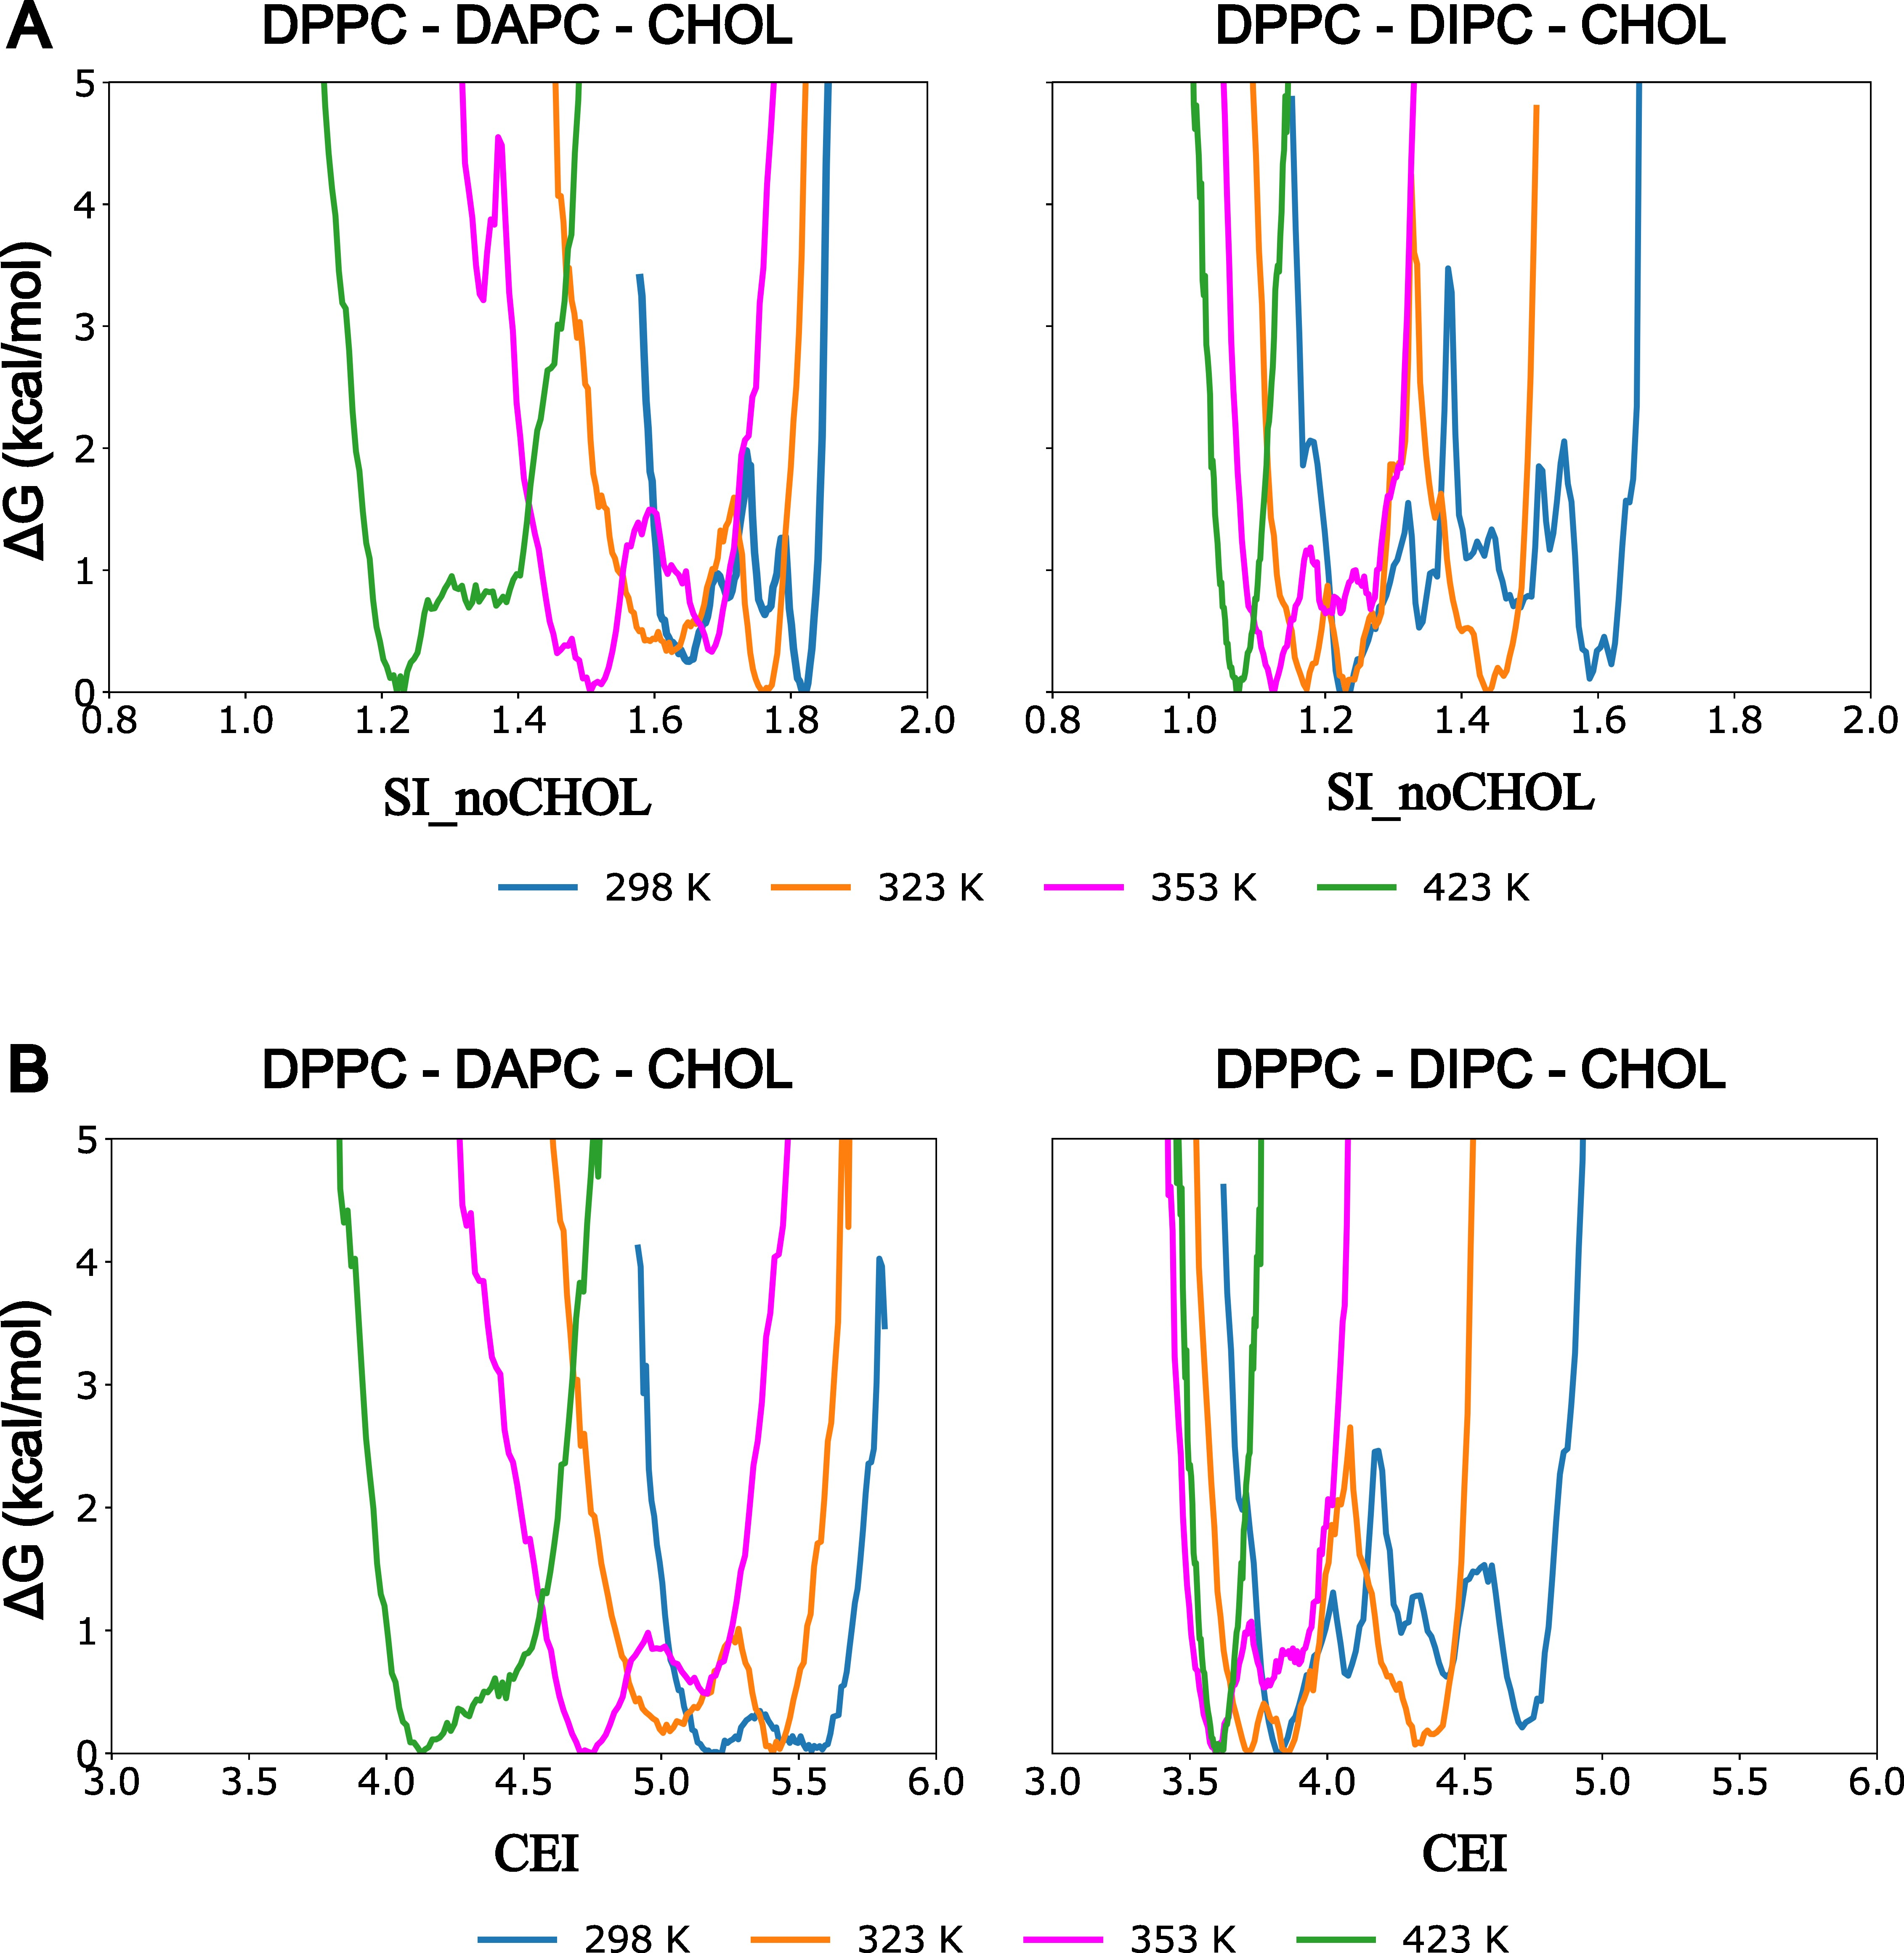
\includegraphics[width=3.25in]{Figures/Main/6/placeholder.jpg}
\caption{A. Free energy landscapes reconstructed using the ensemble of configurations generated during last 10 iterations of FLC-driven WE simulation. The free energy landscape is reconstructed with respect to $\text{SI}_{\text{noCHOL}}$ for DPPC-DAPC-CHOL and DPPC-DIPC-CHOL system respectively. B. The free energy landscape is reconstructed with respect to CEI for DPPC-DAPC-CHOL and DPPC-DIPC-CHOL system respectively. The lines are colored to represent different simulation temperatures}
\label{figs6:view}
\end{figure}

One outcome of WE simulation is the curated ensemble of diverse structures generated by the trajectories.
By construction, WE resampling ensures that the weights associated with these walkers are unbiased.
Thus, we can reuse these weights to examine other variables of choice post-simulation without any need to reweight; this is advantageous, because reweighting is nearly always a lossy procedure.
Assuming the initial configurational distribution relaxed into an equilibrium distribution during the WE simulations (see Discussion), 
we can reconstruct analogous free energy landscapes with collective variable candidates that underperformed for sampling but are otherwise more intuitive to understand.
Fig \ref{figs6:view} A and B show reconstructed free energy landscapes with $\text{SI}_{\text{noCHOL}}$ and CEI by combining the weights from the last ten iterations of the four FLC-generated replicas for each system.

\subsection*{Computing the free energy of separation}

\begin{figure}[hbt!]
\centering
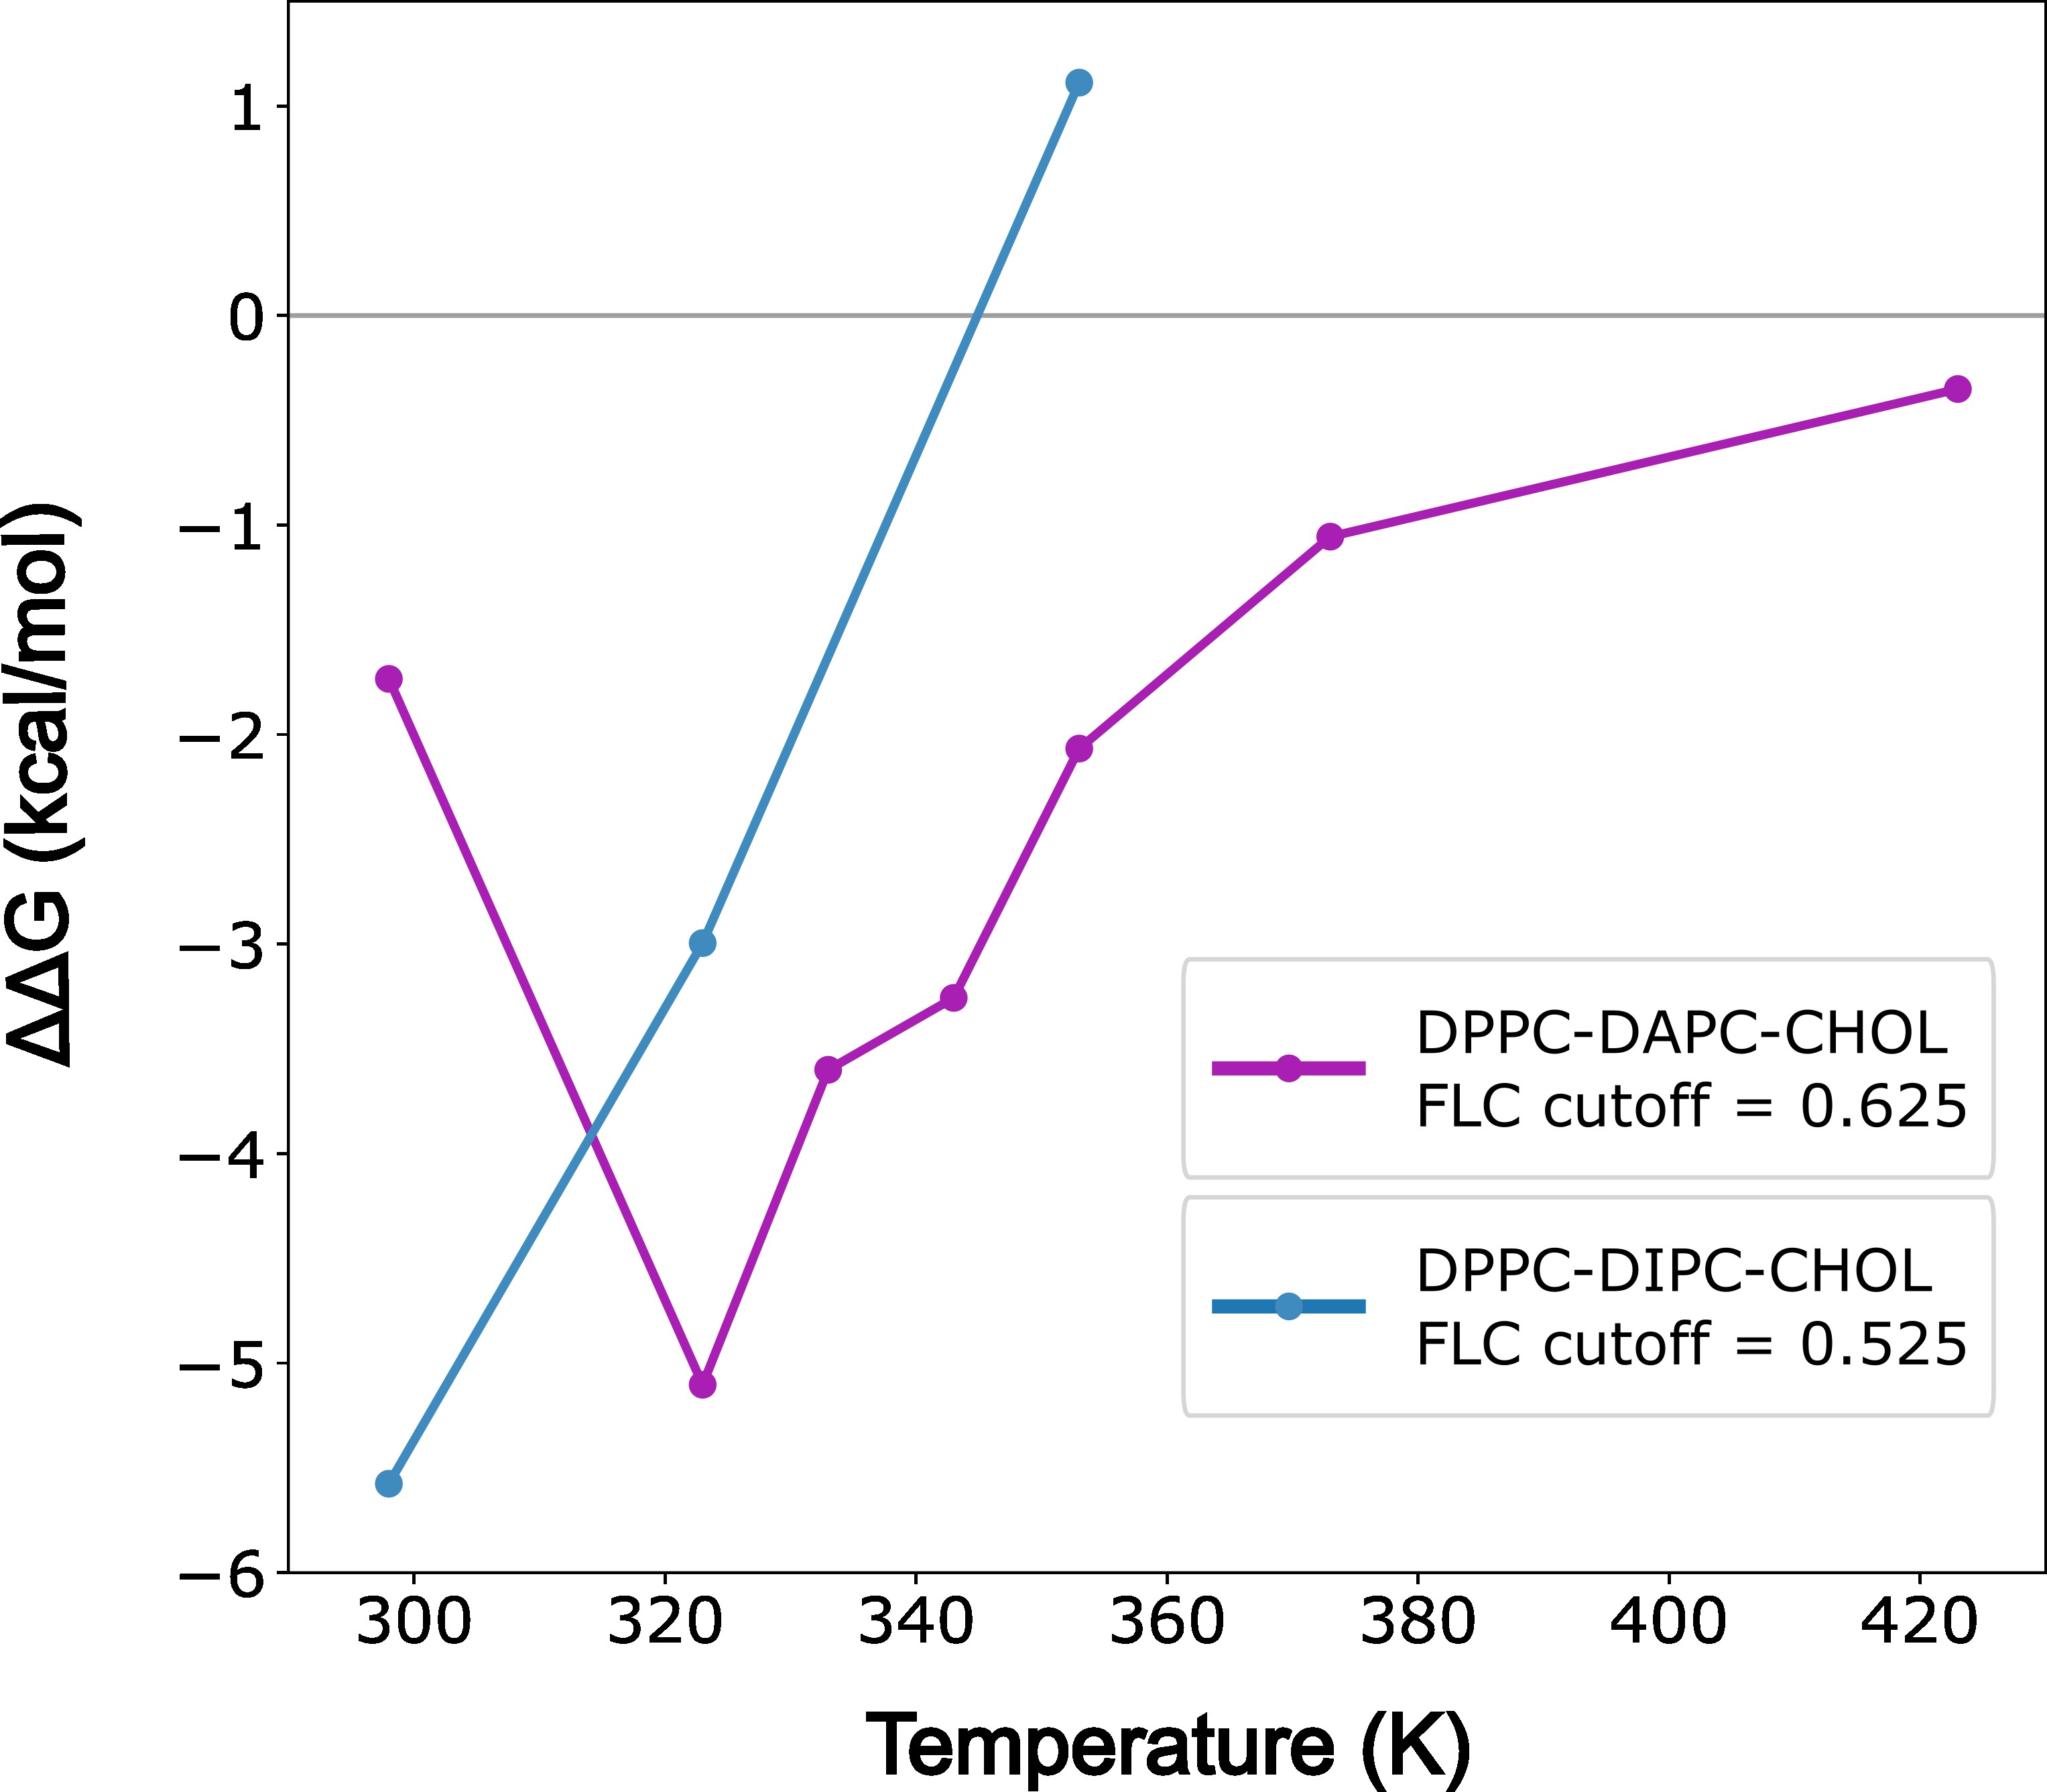
\includegraphics[width=0.5\linewidth]{Figures/Main/7/placeholder.jpg}
\caption{$\Delta\Delta$G profile for DPPC-DAPC-CHOL and DPPC-DIPC-CHOL systems for a given cutoff. Each curve represents $\Delta\Delta$G for the system to transition from mixed to the separated state. Negative values indicate phase coexistence is favored}
\label{figs7:view}
\end{figure}

If we define a cutoff FLC value that separates the well-mixed and phase-separated states, we can compute the free energy change for phase separation as 
\begin{equation}
    \Delta \Delta G_{\text{sep}} = -k_B T \ln \frac{p_{\text{sep}}}{p_{\text{mixed}}}
\end{equation}

One challenge, however, is that the locations of the basins shift with temperature, as seen in Fig \ref{figs5:view}A, and
at higher temperatures, the notion of two states -- mixed and separated -- breaks down as the double-well behavior of free energy curves turns into a single well. 
One trivial solution would be to define a rigid FLC cutoff for a system.
However, a caveat for this approach, as seen in Fig \ref{figs5:view} A, is that the free energy basin for a specific state of the DPPC-DIPC-CHOL system is different for the respective state basin for the DPPC-DAPC-CHOL system.
For this reason, devising a rigorous systematic way to define the separator between the states will require more investigation. In the mean time, we use visual inspection to define FLC cutoffs of 0.525 and 0.625 for the DPPC-DIPC-CHOL and DPPC-DAPC-CHOL systems respectively.
Figure \ref{figs7:view} shows the $\Delta\Delta$G curve for the DPPC-DAPC-CHOL and DPPC-DIPC-CHOL systems as a function of temperature for respective FLC cutoff. In principle, one can identify a melting temperature $T_m$ as the temperature at which $\Delta\Delta G_{\text{sep}}=0$; however, the value derived
in this manner is sensitive to the choice of FLC cutoff, as shown in Supplementary Figure S8.
%TODO : fix this reference to the supplement


\section*{Discussion}

\begin{figure}[hbt!]
\centering

\includegraphics[width=6.5in]{Figures/Main/8/placeholder.jpg}
\caption{Schematic representation of the proposed FLOPSS pipeline. The pipeline is modular. Each module has layers that can be translated to any phase separating system.}
\label{figs8:view}
\end{figure}

Here we propose a proof-of-concept pipeline to construct \textbf{F}ree energy \textbf{L}andscape \textbf{O}f \textbf{P}hase \textbf{S}eparating \textbf{S}ystems (\textbf{FLOPSS}) by realizing multiple transition events using WE strategy.
Even though our systems of interest are lipid bilayers, using appropriate model resolution and collective variables can potentially generalize this pipeline to any system that phase separates.
The modular pipeline is outlined in Figure \ref{figs8:view}, with different sublayers that constitute each module.

The free energy landscapes generated with FLOPSS are consistent with behaviors from the literature, opening up applications to other systems, including asymmetric bilayers, bilayers including peptides or proteins, or all-atom models. We also plan to investigate the effects of finite-sized systems on the phase separation thermodynamics \cite{Pantelopulos2017}. One additional advantage of basing the method on WE is that it can also be used to study the kinetics of phase separation as well as the thermodynamics. One other major area of research is determining whether other collective variables might perform better and allow for less ambiguous procedures for determining $\Delta\Delta G_\text{sep}$. Finally, many of the details of the pipeline could be further optimized, especially those associated with the WE runs themselves.

\section*{Conclusion}

In this work, we have proposed a simple yet efficient collective variable that
simultaneously tracks phase separation and drives WE simulation, ensuring
sufficient state crossing with reasonable convergence of configurational
distribution. We give yet another example of why collective variable choice is
crucial for the success of enhanced sampling protocols, and that there can be
considerable gaps in performance between otherwise reasonable variables. Thus,
a more thorough and systematic analysis of the sensitivity of WE simulation on
the choice of collective variable is needed and is unfortunately beyond the
scope of this work.

In summary, we have developed and validated a new framework that can directly compute the thermodynamics associated with lipid phase separation from simulation.
We have also demonstrated the potential reuse of a reasonably well-converged WE simulation driven by a good collective variable to explore other variables, which otherwise constitute a poor choice for driving WE simulation.
Thus, we can increase the effectiveness of WE simulation without compromising on computational cost.
Moreover, we also showcase the potential of FLOPSS to construct a $\Delta\Delta$G profile of the system under study to investigate the melting properties.
We want to highlight that by generalizing the collective variable FLC to track clustering in 3D space, FLOPSS can in principle be extended to other instances of biological phase separation.


\section*{Acknowledgements}

This work is dedicated to Dr. Klaus Gawrisch, who has inpsired much of our interests in lipid bilayers. The authors thank the Center for Integrated Research Computing (CIRC) at the University of Rochester for providing
computational resources and technical support. The authors also thank Prof. Lillian Chong and Prof. Daniel Zuckerman and
WESTPA Data and Dev club for insights. The authors thank Anthony Bogetti, Jeremy Leung, John Russo, Dr. Sreyoshi Sur, and Dr. Tod D. Romo for their support.
This work was supported by grant R21GM138970 (to A.G.) from the National Institutes of Health.


% ------------------------- %
% Uncomment if using bibtex (default)
\bibliography{PhaseSeparationArticle}

\end{document}